\documentclass{VUMIFPSkursinis}
\usepackage{algorithmicx}
\usepackage{algorithm}
\usepackage{algpseudocode}
\usepackage{amsfonts}
\usepackage{amsmath}
\usepackage{bm}
\usepackage{caption}
\usepackage{color}
\usepackage{float}
\usepackage{graphicx}
\usepackage{listings}
\usepackage{float}
\usepackage{subfig}
\usepackage{wrapfig}
\usepackage[hidelinks]{hyperref}
\usepackage{todonotes}
\usepackage{xcolor}
% Titulinio aprašas
\university{Vilniaus universitetas}
\faculty{Matematikos ir informatikos fakultetas}
\department{}
\papertype{Programų kūrimo proceso laboratorinis darbas}
\title{Įmonės ,,Mėnuliukų technologijos" programų kūrimo proceso aprašas}
\titleineng{Description of the development process of the ,,Mėnuliukų technologijos" company}
\status{4 kurso 3 grupės studentai}
\author{Mėnuliukai}


\supervisor{Saulius Ragaišis, Doc., Dr.}
\date{Vilnius – \the\year}

% Nustatymai
% \setmainfont{Palemonas}   % Pakeisti teksto šriftą į Palemonas (turi būti įdiegtas sistemoje)
\bibliography{bibliografija}

\begin{document}
\maketitle

\tableofcontents
	\section{Vertinimo apimtis}
		\begin{itemize}
			\item{Vertinta pagal - CMMI-DEV, V1.3}
			\item{Vertinimo apimtis - visa antrame darbe pagerinta organizacija.}
			\item{Aukščiausias vertinamas gebėjimo lygis - maksimalus kurį gali pasiekti procesų sritis.}
			\item{Vertinamos procesų sritys:
				\begin{enumerate}
					\item{Causal Analysis and Resolution}
					\item{Configuration Management}
					\item{Integrated Project Management}
					\item{Organizational Process Definition}
					\item{Organizational Performance Management}
					\item{Organizational Process Performance}
					\item{Project Planning}
					\item{Process and Product Quality Assurance}
					\item{Quantitive Project Management}
					\item{Requirement Development}
					\item{Requirements Management}
					\item{Technical Solution}
					\item{Validation}
					\item{Verification}
				\end{enumerate}
			}
		\end{itemize}
	\section{Vertinimo rezultatai prieš pagerinimą}
	\begin{figure}[!htbp]
		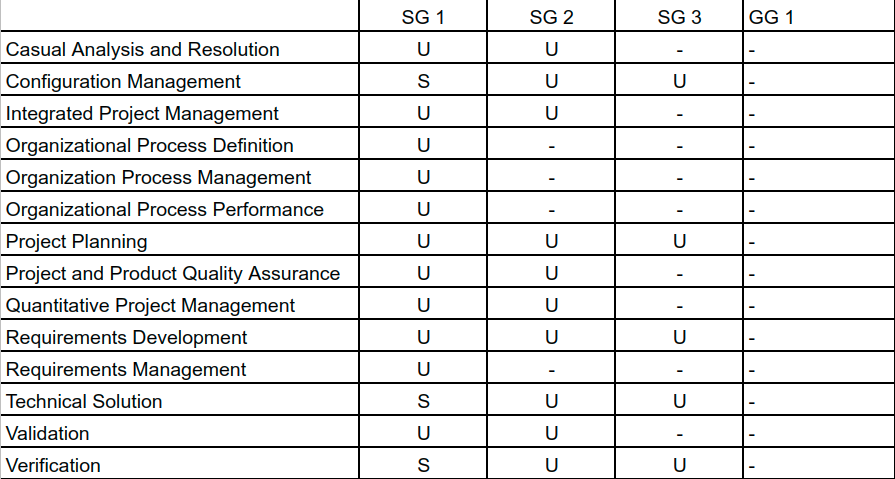
\includegraphics[scale=0.55]{img/profilisPriesLentele}
		\caption{CMMI vertinimo rezultatų gebėjimo profilis prieš pagerinimą lentelėje} % Antraštė įterpiama po paveikslėlio
		\label{img:ProfilisPries}
	\end{figure}
	\begin{figure}[!htbp]
		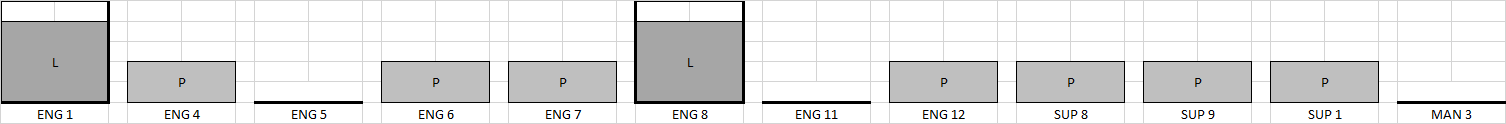
\includegraphics[scale=0.8]{img/ProfilisPries}
		\caption{CMMI vertinimo rezultatų gebėjimo profilis prieš pagerinimą} % Antraštė įterpiama po paveikslėlio
		\label{img:ProfilisPries}
	\end{figure}
	\section{Technical solution}
		\subsection{Pagerinimas}
			\subsubsection{Proceso aprašymas po pagerinimo}
		\subsection{NI PI LI FI atitikimas po pagerinimo}
	\section{Verification}
		Buvo nutarta, kad įmonėje vertifikaciją yra viena iš labiau išvystytų aspektų todėl norėjom jį dar labiau pastumti į priekį, kad ši sritis tarnautų dar ilgą laiką. 
		Taip pat pamanėme, kad jeigu verifikacijos veikla įmonėje būtų išvystyta pilniau, būtų mažiau pataisymų, perdarimų ir konfliktų su užsakovų dėl produkto kuris neatitiktų reikalavimų.
		\subsection{Pagerinimas}
			\subsubsection{Proceso aprašymas po pagerinimo}
		\subsection{NI PI LI FI atitikimas po pagerinimo}
	\section{Configuration management}
		\subsection{Pagerinimas}
			\subsubsection{Proceso aprašymas po pagerinimo}
		\subsection{NI PI LI FI atitikimas po pagerinimo}
	\section{Vertinimo rezultatai po pagerinimo}
	\section{Rezultatai ir išvados}

\end{document}
